\documentclass{report}
\usepackage[utf8]{inputenc}
\usepackage{amsmath}
\usepackage{graphicx}
\usepackage{hyperref}
\parindent=0pt
\usepackage[a4paper, total={165mm, 235mm}]{geometry}
\usepackage[section]{placeins}
\usepackage{enumitem}
\usepackage{caption}
\usepackage{parskip}
\usepackage{multirow}
\usepackage{biblatex}
\addbibresource{Bibliography.bib}
\usepackage{wrapfig}

\title{PySPI for Persistent Sources}
\author{Möller, Julius}
\date{June 2023}

\begin{document}

\begin{titlepage}
    
    
\includegraphics[height=1cm]{Images/General/MPE_logo_189x180px.jpg}
    \hfill
    
\includegraphics[height=1cm]{Images/General/PH.pdf}
    
\includegraphics[height=1cm]{Images/General/tumlogo.pdf}

    \begin{center}
        \vspace{1cm}
        \large

        Max Planck Institute for Extraterrestrial Physics
        

        \vspace{1.5cm}
        \large
        Thesis for Master of Science in Astrophysics
        
        \vspace{3cm}
        \Huge
        PySpi for Persistent Sources
        
        \vspace{3cm}
        
        \LARGE
        Julius Möller
        
        \vspace{1.5cm}
        \large
        June 2023
        
        
        \vspace{6.5cm}
        
        
        
        \large
        Technische Universität München

        Fakultät für Physik
        
        
        
    \end{center}
\end{titlepage}


\tableofcontents

\pagebreak

\chapter{Introduction}
\label{Introduction}
\section{About INTEGRAL}


\begin{wrapfigure}{r}{0.50\textwidth}
  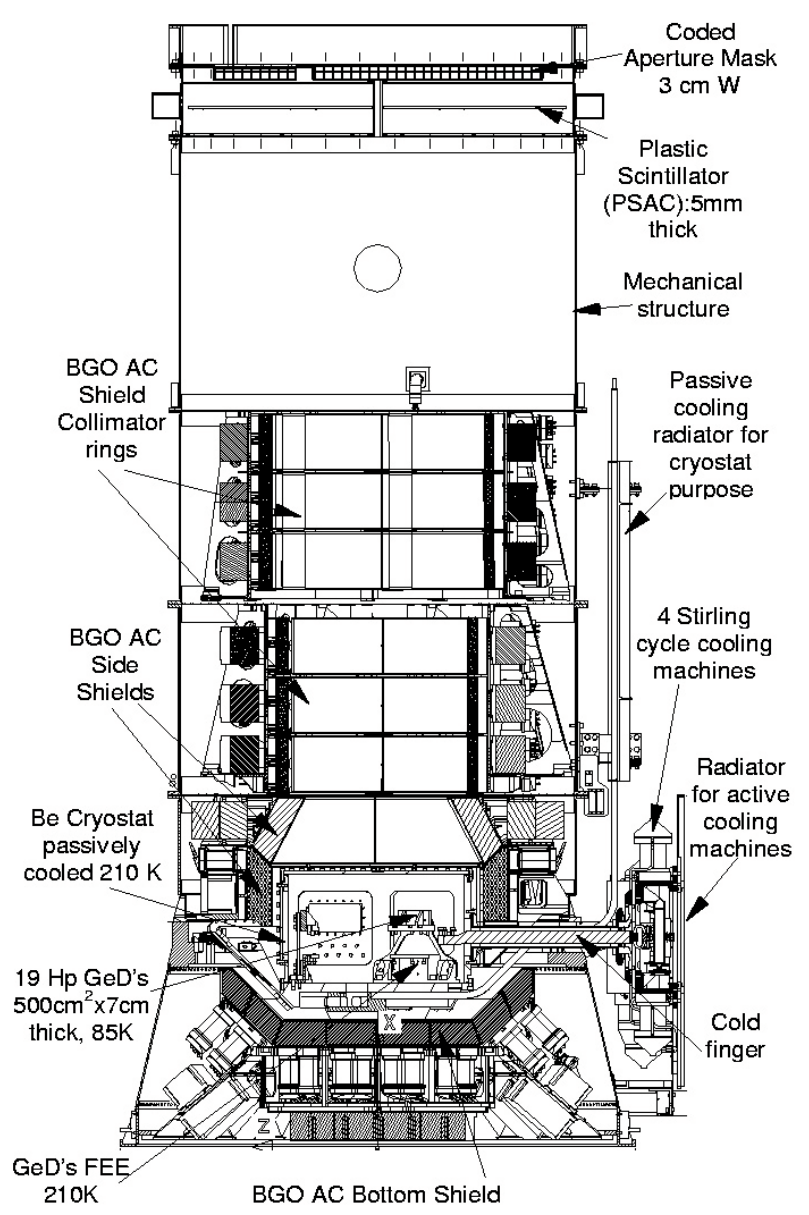
\includegraphics[width=\linewidth]{Images/General/SPI_cut_view_verdenne_2003.PNG}
  \vspace{-20pt}
  \caption{Cut-out view of the SPI spectrometer \cite{refId0}.}
  \vspace{-20pt}
  \label{SPI cut view}
\end{wrapfigure}


The INTErnational Gamma-Ray Astrophysics Laboratory (INTEGRAL) is an ESA space telescope with contributions from NASA and the RKA. Its mission began on October 17, 2002, when a Proton-DM2 rocket launched it from the Russian Baikonur spaceport in Kazakhstan into a 3-day, highly elliptical orbit with an apogee of 153000km and a perigee of 9000km, although this has not remained constant over the course of its lifetime. This places INTEGRAL mostly above radiation belts that would cause high instrumental backgrounds from charged-particle activation, and is why data collecting is halted during hours of close Earth-proximity. Initially, INTEGRAL had a 2+3-year planned lifetime, which it has greatly exceeded due to its lower than expected fuel consumption. Since then, its science operations have been repeatedly extended, currently up to the end of 2024, with some difficulties along the way such as its failed thrusters in July 2020 (compensated through the use of reaction wheels) and an uncontrolled tumbling caused by a single event upset in September 2021. The satellite is predicted to reenter Earth's atmosphere in 2029.



Onboard INTEGRAL are two main instruments: the Imager on-Board the INTEGRAL Satellite (IBIS) and the SPectrometer of INTEGRAL (SPI). IBIS specializes in being able to locate sources effectively. With an angular resolution of 12 arcmin, it can locate bright sources with arcmin precision in its $9^\circ \times 9^\circ$ field of view, and covers an energy range from 15keV to 10MeV. 

\subsection{About SPI}




SPI, the instrument used in this thesis and illustrated in figure \ref{SPI cut view}, specializes in its detailed energy resolution. At 1.3MeV, it is able to resolve energies with 2.5keV precision. It has a field of view of $16^\circ$ and an energy range covering 20keV to 8MeV. One decisive advantage SPI has in comparison to many comparable instruments is that its response matrices are based on extensive ground calibrations and Monte-Carlo simulations, as opposed to relying on astronomical sources such as the Crab Nebula.





\subsubsection*{Detectors}
SPIs detectors are composed of an hexagonal array of 19 reverse-electrode n-type germanium detectors. With a mean crystal weight of 951g and mean volume of $178\text{cm}^3$, the total geometrical area for a flux parallel to the axis is $508\text{cm}^2$. Under normal working conditions, a voltage of 4000V is applied to each detector independently, and this voltage is variable between zero and 5000V. 

The germanium detectors require temperatures below 100K to work effectively, preferably as low as 85K in order to slow the effects of radiation damage. To accomplish this, SPI is equipped with an active cryogenic system. The Ge array is fixed on a Be plate, which is placed inside the cryostat. The plate is connected to the Stirling cycle cryocoolers to provide active cooling. 

Despite the low temperatures and hexagonal design to reduce the probability of hole traps in the semiconductor, radiation damage will inevitably accumulate over the course of a year or more. To combat this issue the detectors can undergo an annealing process, in which they are held at a temperature of $105^\circ \text{C}$ over the course of one or two days, depending on the damage. An annealing process of two days is enough to fully recover the energy resolution after radiation damage leading to a 20\% increase in the FWHM at 1.3MeV \cite{refId0}.

Each detector is connected to a preamplifier, which outputs the charge integrated signal (proportional to the measured energy) and the PSD signal (see below) to the detectors respective electronic chains for processing.

\subsubsection*{Pulse Shape Discrimination electronics (PSD)}



In order to suppress background events, SPI is equipped with Pulse Shape Discrimination (PSD) electronics. The idea is that localized beta decays in the detector material, which would otherwise be indistinguishable from photon energy deposits, only interact in a small volume of the detector, resulting in a single current pulse in the preamplifier. Gamma-rays, which primarily deposit energy via multiple compton scatterings in the detector volume, thus lead to a broader signal. 

Each detector is connected to its own PSD electronic system, which is only triggered in a certain energy range. The lower level threshold (LLD) is configurable, and has been varied between 400keV and 750keV over the missions lifetime, where as the upper level threshold (ULD) is fixed at around 8MeV. Naturally, processing and analyzing the shape of a signal takes time, and when another event is measured within this time it is stored without any PSD information. The PSD electronics thus have an efficiency that can be approximated around 85\% \cite{Roques}.



\subsubsection*{Anticoincidence shield (ACS)}

\begin{wrapfigure}{R}{0.30\textwidth}
  \vspace{-20pt}
  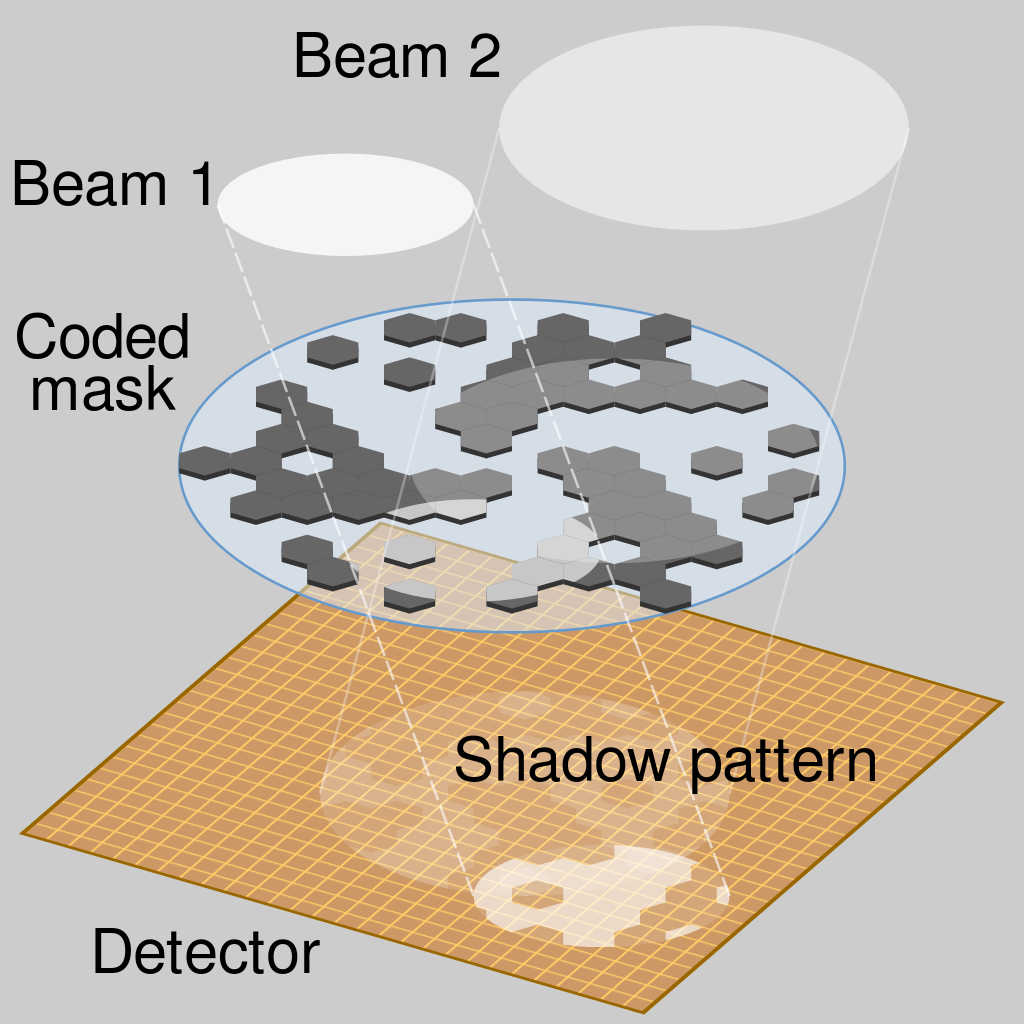
\includegraphics[width=\linewidth]{Images/General/HURA_hexagonal_coded_aperture_mask_principle.svg.png}
  \vspace{-20pt}
  \caption{The effect of SPIs mask on incoming source beams \cite{HURA}.}
  \vspace{-20pt}
  \label{HURA}
\end{wrapfigure}

To further prevent unnecessary background counts in the detectors an anticoincidence shield (ACS) is installed around various of SPIs components (see figure \ref{SPI cut view}). It consists of 91 BGO crystals with a volume of approximately $790\text{cm}^3$ each. Whenever an event is measured simultaneously in the ACS and in the Ge detectors it is vetoed. 



\subsubsection*{Mask}



\begin{figure}[]
  \centering
  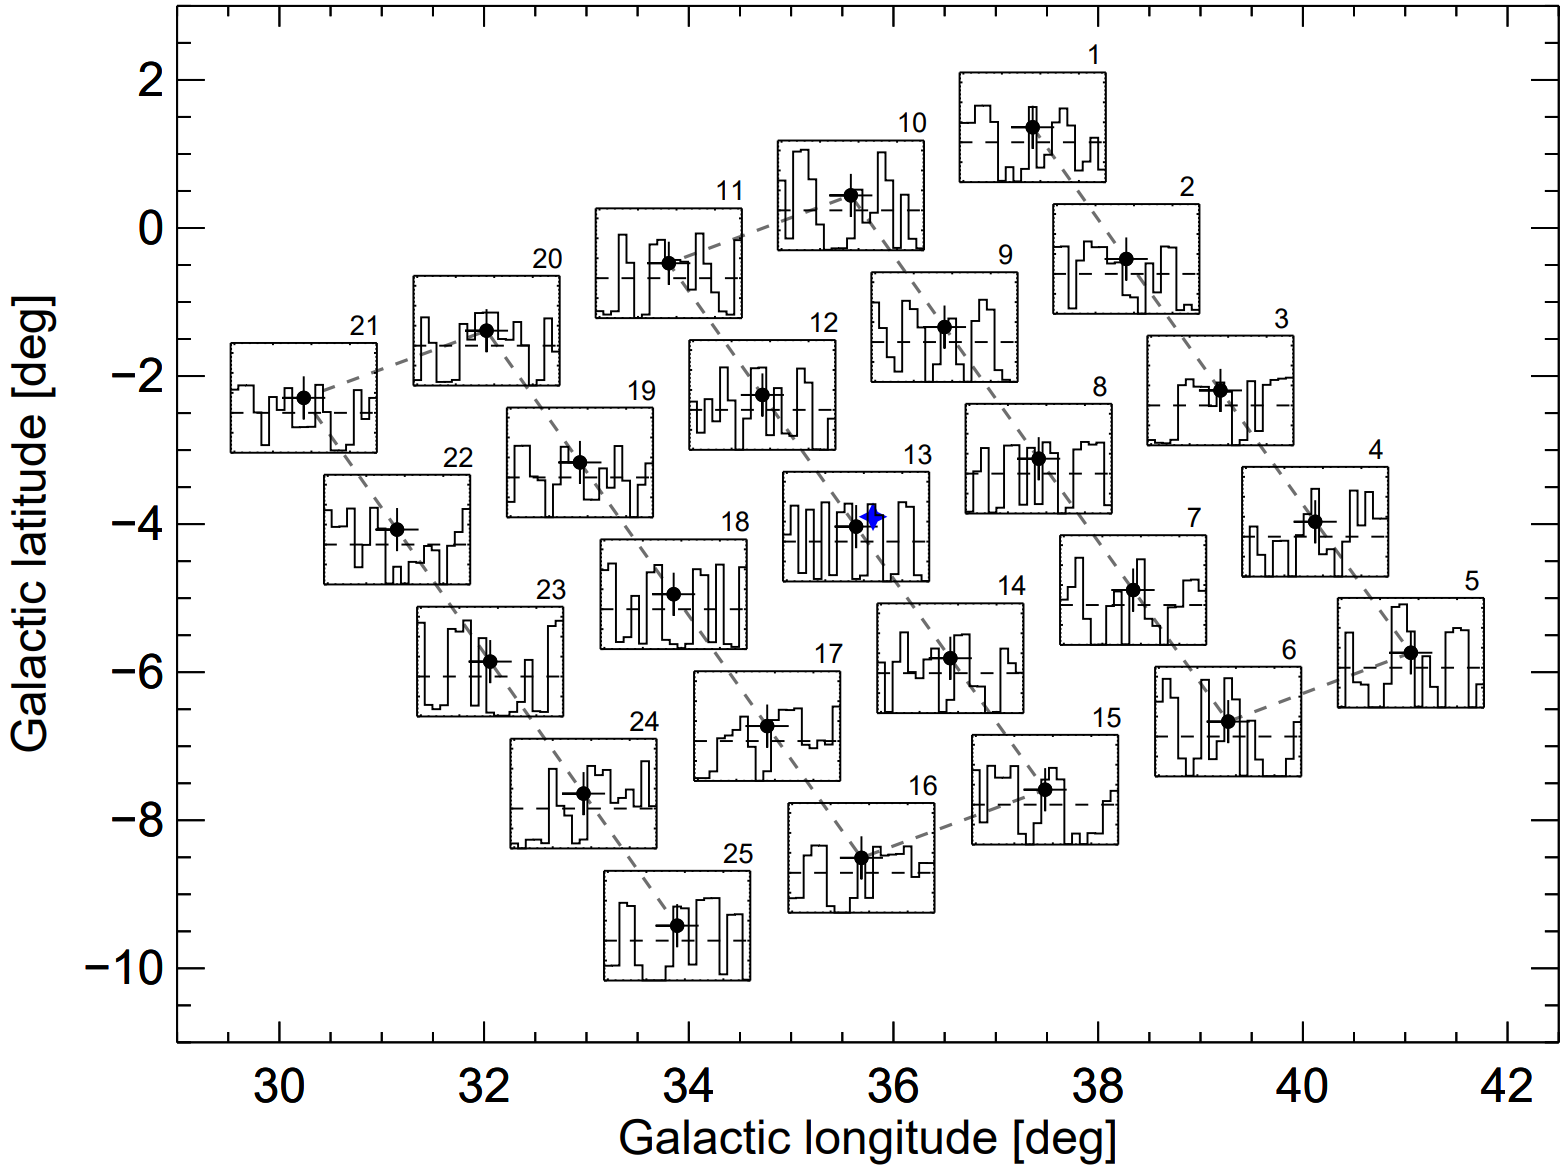
\includegraphics[width=\textwidth]{Images/General/Siegert_PHD_Pointings_pattern.PNG}
  \caption{A typical SPI $5\times5$ grid pointing pattern, each $2.1^\circ$ apart, marked with black dots and sequence number. The blue star in the center represents a celestial source, and the inset panels show the relative detector patterns from the celestial source. A close-up of pointing 13 is shown in figure \ref{spegert_pointings_pattern_close_up}. \cite{dissertation}}
  \label{spegert_pointings_pattern}
\end{figure}

\begin{figure}[]
  \centering
  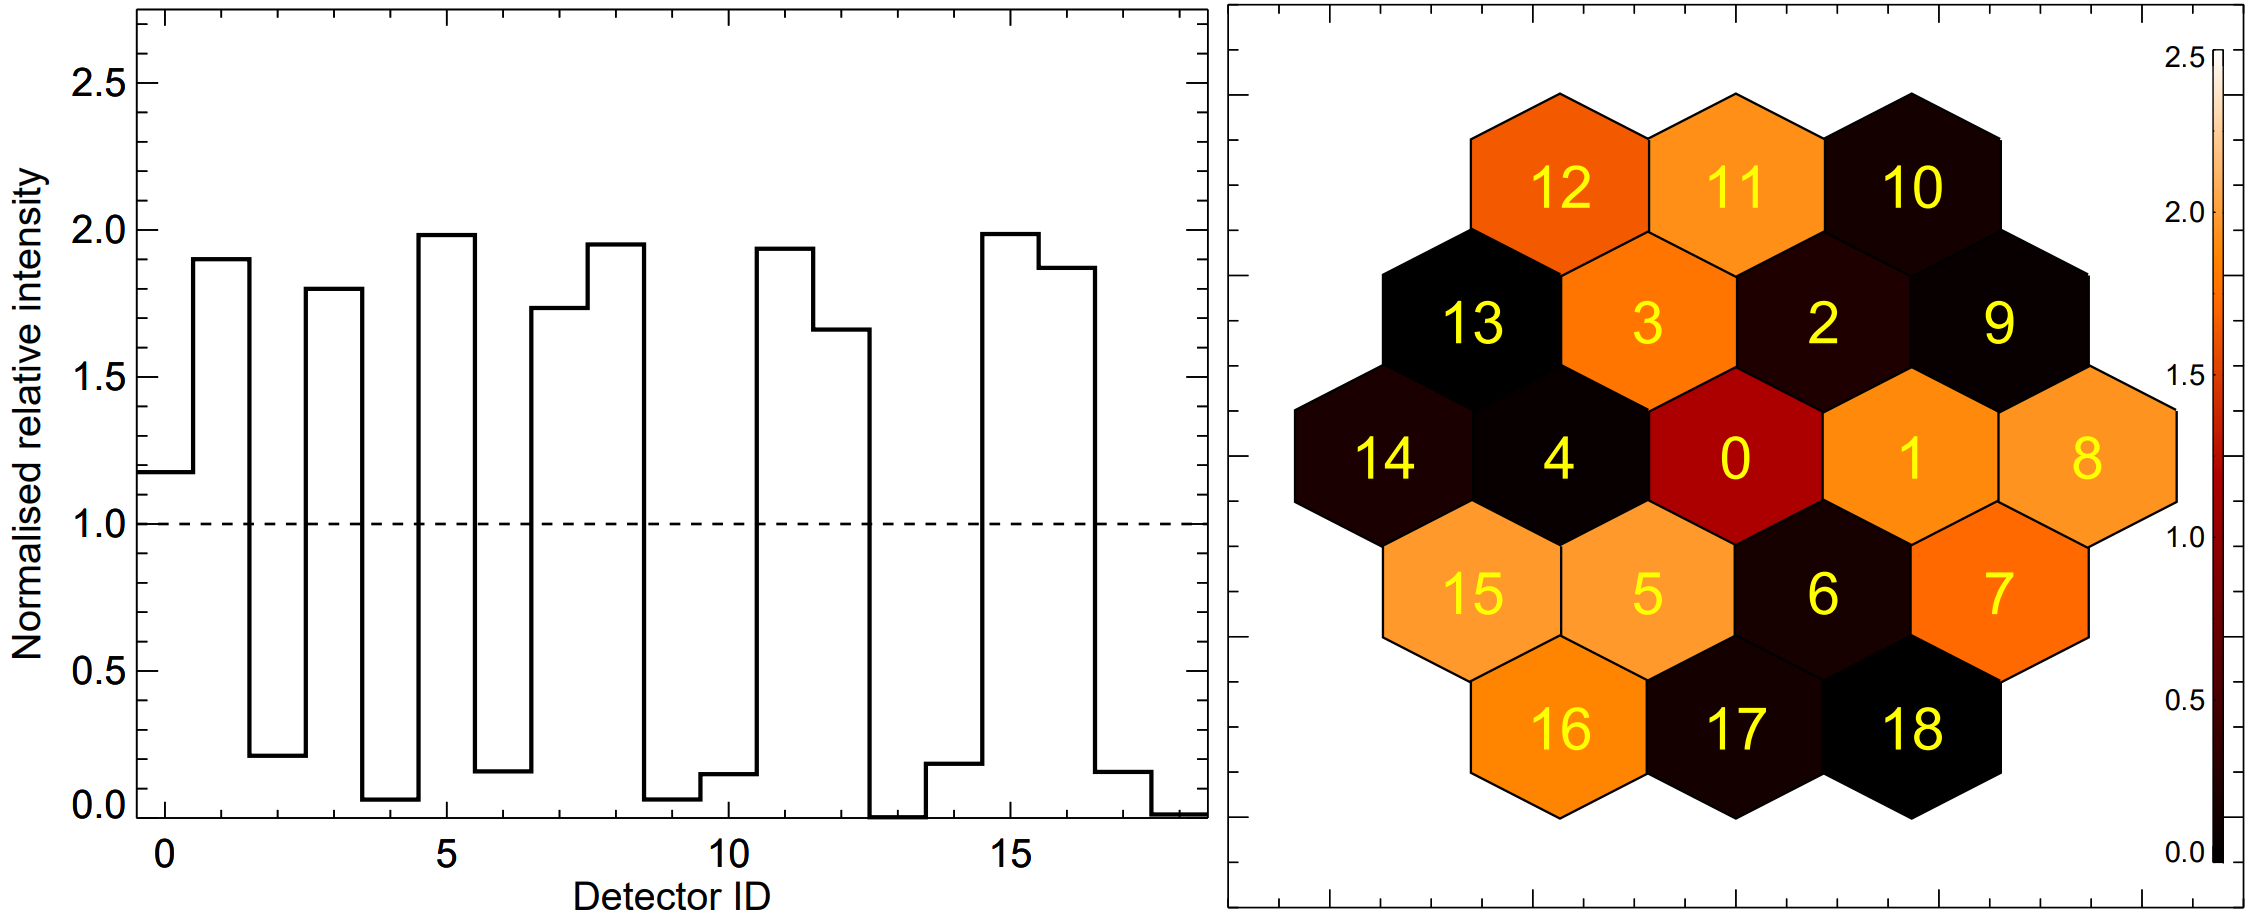
\includegraphics[width=\textwidth]{Images/General/Siegert_PHD_P13.PNG}
  \caption{A close-up of pointing 13 from figure \ref{spegert_pointings_pattern}. On the left we see the relative detector pattern caused by the source in a step plot, and on the right we see the same information displayed as a shadowgram on the detector array. \cite{dissertation}}
  \label{spegert_pointings_pattern_close_up}
\end{figure}

Before any photons can reach the array of detectors, they must pass through the coded aperture mask made of a 3cm thick tungsten alloy, located 1.71m above. The $120^\circ$ rotationally symmetric mask is composed of 127 hexagonal tiles (63 opaque and 64 transparent to gamma radiation in the operating energy range) measuring 60mm side to side, and is inscribed within a circle with 720mm diameter. The effect that the mask has on incoming source beams is illustrated in figure \ref{HURA}, and the way this might influence the number of source counts measured in the detector array is visualized for an example source in figures \ref{spegert_pointings_pattern} and \ref{spegert_pointings_pattern_close_up}. This illustrates how we may infer both the source spectrum and position from the detector counts using multiple offset pointings of an astronomical source.




\subsubsection*{Event Types}
\begin{wrapfigure}{R}{0.55\textwidth}
  \vspace{-20pt}
  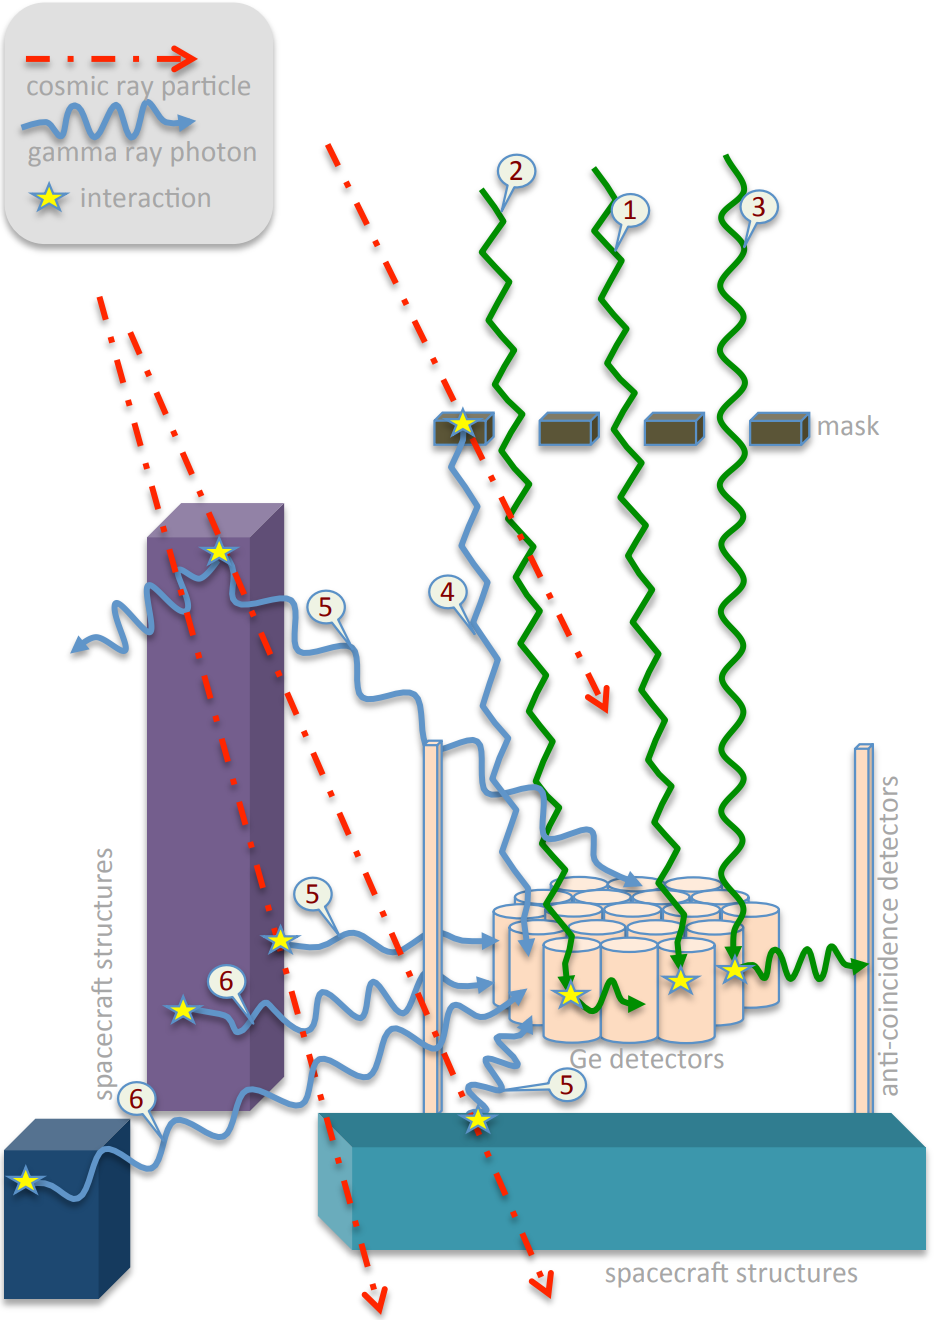
\includegraphics[width=\linewidth]{Images/General/SPI_event_types_roland_2017.PNG}
  \caption{Illustrations of different event types measured by SPI. Incoming source photons (green) may be absorbed in one detector (1), multiple detectors (2), or be self-vetoed by interacting with the ACS (3). Cosmic particles may interact with surrounding structures, resulting in background photons (blue)(4,5,6). Although the ACS helps suppress these events, they still occur. \cite{refId2}}
  \vspace{-50pt}
  \label{event_types}
\end{wrapfigure}

Figure \ref{event_types} shows some of the different event types measured by SPI. These are generally classified in the following categories:

\begin{itemize}
  \item Single Events (SE) - only one of the Ge detectors measured an energy deposit in the relevant time frame. Ideally this photon is fully absorbed in the detector, although there is no way of confirming this.
  \item Multiple Events (ME) - multiple Ge Detectors measured an energy deposit simultaneously. Ideally this is caused by a photon compton scattering to another detector (or multiple detectors), where it is fully absorbed. Again, there is no way of confirming this the photon is fully absorbed or that the measured energies were not coincident from multiple sources.
  \item Pulse Shape Discriminated Events (PE) - A SE for which the PSD electronics also triggered. Since each detector is equipped with its own PSD electronics chain, only SEs can be pulse shape discriminated. Another effect of this implementation is that the SE spectrum will have a reduced count rates in the PSD energy range, where SEs are PSD flagged and thus "removed" from the SE spectrum. 
\end{itemize}

Although the ACS does help with suppressing background and non-fully absorbed photons, it cannot guarantee  anything. In fact, a very large portion of SPIs measured counts are background counts. 

\subsubsection*{Spurious Events}
SPI also suffers from so called spurious events. These may occur when high-energy deposits are made in the germanium detectors. The analog electronics can become saturated and, due to reasons better explained elsewhere \cite{Roques}, low energy counts will be displaced toward higher energies. However, it has been found that the PSD electronics chain does not suffer from the same issues. This is why it is recommended to use only PEs in the PSD energy domain, and not SEs. 


\section{About Spimodfit}



Given the complexities discussed above, and many more not discussed, it is clear that working with SPI data is no trivial task. Although SPIs Instrument Response Function (IRF) are readily available to be used, there is no stand-alone background model. Since the background counts dominate source counts in almost all circumstances, it is no surprise that several independent methods to analyze SPI data have been developed. One such method is Spimodfit, developed primarily by Thomas Siegert at MPE \cite{refId1} \cite{SMF_Cookbook}.

\begin{wrapfigure}{R}{0.55\textwidth}
  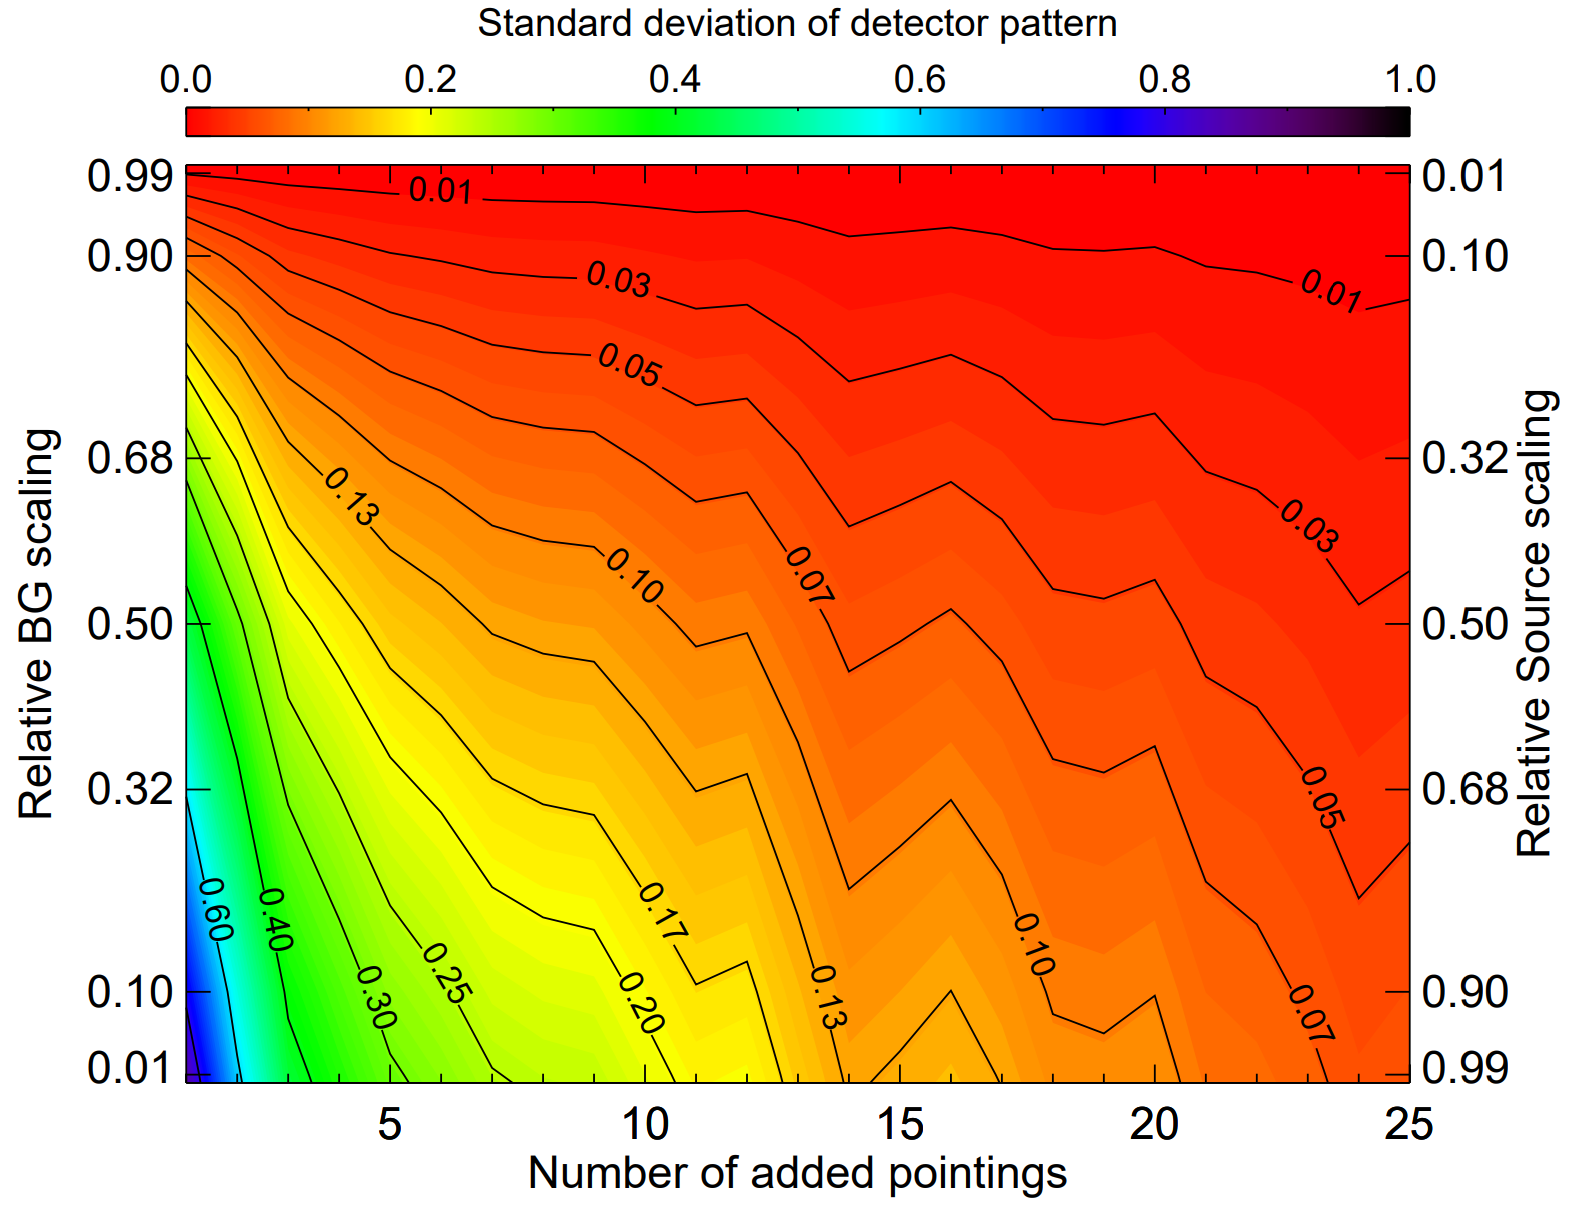
\includegraphics[width=\linewidth]{Images/General/SMF_background_pattern_siegert_2019.PNG}
  \caption{The standard deviation of detector patterns as a function of the number of pointings and the source to background intensity. We see that even very bright sources become almost entirely washed out given enough pointings, and only the sum of the background detector patterns remains. \cite{refId1}}
  \vspace{-0pt}
  \label{smf_background_model_idea}
  \vspace{-5pt}
\end{wrapfigure}

In order to create Spimodfit a detailed background and response database had to be constructed first. The fundamental idea that allows this background database to work is that the detector count-rate patterns of individual isotopes stay constant on all timescales. This means that every process that leads to background counts creates some specific, energy dependent pattern in the detector array which stays constant. These processes are split into parameters for continuum processes as well as many $\gamma$-ray lines. The intensities of these different patterns created by the processes may vary, which is why they are fitted to the relevant count-spectra per energy bin in order to create the background spectrum used in every analysis. This requires one to have knowledge of what the different patterns are. Hence, a database of the detector patterns was created by adding many SPI pointings together over relevant timescales, so that any sources in the pointings are washed out and only the detector patterns remain (see figure \ref{smf_background_model_idea}). Naturally, this very brief description of the Spimodfit background model given here skips over many details and complexities that had to be taken into consideration.

Spimodfit will be used extensively in this thesis as a reference point regarding SPI data fitting.



\section{PySPI and the Goal of this Thesis}
PySPI is a python analysis framework for Gamma-Ray Burst (GRB) data from SPI \cite{Biltzinger2022}. It is designed to take user inputs like the time of the GRB and energy bins, automatically download relevant data files, and to construct a response and time series, which can then be used as a plugin for 3ML \cite{3ml}.

Momentarily, PySPI is only built to work with transient sources. The goal of this thesis is to extend PySPIs functionality to be able to analyze persistent sources as well. Unlike transient sources, whose time-sensitive nature circumvents the need for an accurate background description, persistent sources are not so easily distinguished from background counts and thus do necessitate a way to deal with SPIs dominant background.

\chapter{Theory and Simulation}

\section{General Procedure} \label{General Procedure}
In contrast to previous approaches to working with INTEGRAL SPI, the method of analyzing SPI data developed for this thesis does not attempt to construct a background model, and instead uses a profile likelihood to eliminate its effect in the source model fit. The underlying assumption that allows this to work is that background count rates in each energy bin per detector remain constant for temporally and spatially near SPI Science Windows (SCWs) (also called pointings). Neighboring SCWs are thus grouped into clusters of assumed constant background count-rates, allowing for a source model to be fitted to the data using the likelihood calculations described below. Just like in chapter \ref{Introduction}, we distinguish between source counts, which describe all detected events directly originating from astronomical objects considered in our source model, and background counts, which describe all other detector events.

\subsection{Likelihood Calculation}

Once we have split our set of SCWs into clusters within which we claim the assumption of constant background to be true and have defined a source model, a likelihood value can be calculated for each energy bin of each detector in each cluster. If one energy bin of one detector in one SCW with measuring time $t$ has a source count rate $s$ and a background count rate $b$, the probability $P$ of measuring $C$ counts follows a Poisson distribution:
\begin{equation}
    P(C \vert b, s, t) = \frac{\left( t \left( b + s \right) \right) ^C \text{exp}\left( -t \left( b+s\right)\right)}{C!}
\end{equation}

Equivalent energy bins in the same cluster are assumed to have the same background count rate $b$, so that the probability of measuring $C_1$ counts in one SCW and $C_2$ counts in another SCW is simply:

\begin{equation}
    P(C_1, C_2 \vert b, s_1, t_1, s_2, t_2) = P(C_1 \vert b, s_1, t_1) \cdot P(C_2 \vert b, s_2, t_2)
\end{equation}

The likelihood $\mathcal{L}$ for any energy bin of a detector within a cluster depends on all equivalent energy bins in that cluster, i.e. one term for each SCW in the cluster. If we have cluster of size two, the likelihood is described by:

\begin{equation}\label{log likelihood}
    \text{ln}\mathcal{L}(C_1, C_2, t_1, t_2\vert b, s_1 s_2) = \text{ln}P(C_1 \vert b, s_1, t_1) + \text{ln}P(C_2 \vert b, s_2, t_2)
\end{equation}

This expression allows us to solve for the probability distribution of $b$. A full and mathematically correct treatment of the background parameter $b$ turns out to be very cumbersome with only marginal benefits. Hence, the profile likelihood is used by simply solving for the background count rate value $b_M$ which maximizes the likelihood. This is easily done by setting the derivative of equation \ref{log likelihood} to zero and solving for $b$. For a cluster size of two one finds:
\begin{equation}
    b_M = \frac{1}{2} \left[ \frac{C_t}{t_t} - s_t + \sqrt{\left( \frac{C_t}{t_t} - s_t\right)^2 + 4 \left( \frac{C_1s_2+C_2s_1}{t_t}-s_1s_2\right)}\right]
\end{equation}
where $C_t=C_1+C_2$, $s_t=s_1+s_2$, and $t_t=t_1+t_2$. Using this maximum likelihood background $b_M$ finally allows us to compute a likelihood value that is only dependent on the measured counts and the source model:
\begin{equation} \label{log_likelihood final}
    \text{ln}\mathcal{L}(C_1, C_2, b_M, t_1, t_2 \vert s_1, s_2) = \text{ln}P(C_1 \vert b_M, s_1, t_1) + \text{ln}P(C_2 \vert b_M, s_2, t_2)
\end{equation}
The process for clusters with sizes larger than two is analogous. One such likelihood value exists for every energy bin of every detector in every cluster, such that the total likelihood value for any given source model is simply the sum of the logarithmic likelihoods over all energy bins, detectors, and clusters:

\begin{equation} \label{total log likelihood}
  \text{ln}\mathcal{L}_{\text{total}} = \sum_{\text{Clusters}}\sum_{\text{Detectors}}\sum_{\text{Energy-Bins}} \text{ln}\mathcal{L}(C_1, C_2, b_M, t_1, t_2 \vert s_1, s_2)
\end{equation}

Thus the source model may be fitted to the count data by applying an algorithm to maximize the likelihood. In this case Multinest \cite{Feroz_2019} is the bayesian inference algorithm of choice.

\subsection{General Procedure: Summary}

The general procedure for fitting persistent sources with PySPI can thus be summarized in the following steps:
\begin{enumerate}
  \item Select all relevant SCWs to be used in the analysis. Usually this is done on a revolution basis, so that all SCWs from the used INTEGRAL revolutions are included, provided SPIs orientation is sufficiently close to the source in question.
  \item Group the relevant SCWs into clusters. These should preferably have only a small time difference and angular distance in SPIs orientation between them so that the assumption of a constant background rate in every energy bin of every detector is justified. Refer to appendix \ref{Clustering Algorithm} for more details on the clustering algorithm developed for this purpose. In principle, clusters of any size ($>1$) can be used, although only cluster-sizes 2 and 3 have been implemented and tested. Clusters of size 2 are most commonly used since they are generally the easiest to work with due to the constant background assumption and computational speeds.
  \item Set-up a source model to be fitted to the data using the python package astromodels \cite{astromodels}. The built in SPI response function capabilities of PySPI allow one to easily calculate the count rates based on the model.
  \item Set-up equation \ref{total log likelihood} so that the multinest bayesian fitting algorithm can vary the source model parameters to maximize the total likelihood. Then run the fit.
  \item If deemed necessary conduct a posterior predictive check (PPC) analysis (see chapter \ref{sec:PPC Back}) to verify the the fit quality and check if the assumption of constant background rates is well met. It is a common occurrence for some clusters to not have constant (or constant enough) background rates. These are easily identified in the PPC CDFs, so that they may be removed from the list of clusters for the fit to be run again.
\end{enumerate}



\section{Pure Simulation}
Before any real sources are fitted, it makes sense to 


\section{Mixed Simulation and Spimodfit Comparison}


\section{Posterior Predictive Check (PPC) and Background Analysis} \label{sec:PPC Back}




\appendix
\chapter{List of Source Models}

\subsection*{Powerlaw}

\begin{equation} \label{powerlaw}
  f(x) = K \frac{x}{piv}^{index}
\end{equation}

\begin{itemize}
  \item $x$: input energy [keV]
  \item $K$: differnetial flux at the pivot value, i.e. normalization [$\text{keV}^{-1}\text{s}^{-1}\text{cm}^{-2}$]
  \item $piv$: energy for which $K$ gives the normalized flux [keV]
  \item $index$: index of the powerlaw
\end{itemize}




\chapter{Science Window Clustering Algorithm}
\label{Clustering Algorithm}

\nocite{*}
\printbibliography



\end{document}